%% LyX 2.0.5.1 created this file.  For more info, see http://www.lyx.org/.
%% Do not edit unless you really know what you are doing.
\documentclass[usenatbib]{article}
\usepackage[latin9]{inputenc}
\usepackage[a4paper]{geometry}
\geometry{verbose}
\usepackage{color}
\usepackage{graphicx}

\makeatletter

%%%%%%%%%%%%%%%%%%%%%%%%%%%%%% LyX specific LaTeX commands.
%% A simple dot to overcome graphicx limitations
\newcommand{\lyxdot}{.}


%%%%%%%%%%%%%%%%%%%%%%%%%%%%%% Textclass specific LaTeX commands.
\usepackage{jcappub}

%%%%%%%%%%%%%%%%%%%%%%%%%%%%%% User specified LaTeX commands.






%%%%%%%%%%%%%%%%%%%%%%%%%%%%%% LyX specific LaTeX commands.
%% A simple dot to overcome graphicx limitations
%Make my life significantly easier
\global\long\def\bd{{\bm{\delta}}}

\makeatother

\begin{document}

\title{The Maximum Circular Velocity Dependence of Halo Clustering}

\maketitle

\section{Introduction}

XXX


\section{The Simulation}

We use cosmological N-body simulations called the Bolshoi simulation
and the MultiDark simulation, described in XXX and XXX respectively,
to investigate the maximum circular velocity dependence of halo clustering.
The Bolshoi simulation uses $2048^{3}$ particles with a volume of
$(250$$h^{-1}{\rm Mpc})^{3}$, while the MultiDark simulation uses
the same number of particles as the Bolshoi simulation but with a
volume of ($1h^{-1}{\rm Gpc})^{3}$. Both simulations assumes a flat
$\Lambda{\rm CDM}$ model with density parameters $\Omega_{m}=0.27$,
$\Omega_{\Lambda}=0.73$, $\Omega_{b}=0.0469$, and $\sigma_{8}=0.82$,
$n=0.95$, $h=0.70$. (??Do I need to put a name for each constant?)The
details of the simulations are described in XXX. For halo identification,
we use the ROCKSTAR halo finder (XXX) where the halo masses and maximum
circular velocities are computed from bound particles. 

??Should I explain more about what bound particles mean (though my
understanding is vague...) and am not so sure what other ways to define
masses and circular velocity and also how the definitions can make
things different...

??What other information do I need to put here?


\section{The Maximum Circular Velocity Dependence of Halo Clustering}

In this section, we investigate the maximum circular velocity dependence
of halo clustering on both large and small scales. In order to do
that, we compute correlation functions and measure halo biases for
halo samples having different maximum circular velocities. We first
describe how we select halos for each sample and then show how those
samples have different clustering properties.

As shown in Fig. \ref{fig:vmax-mvir}, the maximum circular velocity
and halo mass has tight correlation, and yet the scatter between the
maximum circular velocity and halo mass becomes larger with decreasing
halo masses. In fact, we can compute an expected maximum circular
velocity from halo mass

\begin{equation}
V_{{\rm max}}=0.465M_{{\rm vir}}^{1/3}\sqrt{G(\frac{4}{3}\pi\Delta_{{\rm h}}\rho_{{\rm crit}}\Omega_{m})^{1/3}\frac{c}{{\rm ln(1+c)-c/(1+c)}}},\label{eq:vmax-mvir}
\end{equation}
where $V_{{\rm max}}$ is the maximum circular velocity and $M_{{\rm vir}}$
is the halo mass, $G$ is the gravitational constant, $\Delta_{{\rm h}}$
is XXX, and $c$ is the concentration parameter. To obtain Eq. \ref{eq:vmax-mvir},
we use the concentration of 
\begin{equation}
{\rm log}_{10}c=-0.097{\rm log_{10}M_{vir}}+2.148.
\end{equation}
(??Ask Frank how he obtain this concentration value and why this is
a reasonable value) \textcolor{black}{In Fig. \ref{fig:vmax-mvir},
this $V_{{\rm max}}-M_{{\rm vir}}$ relation with the above concentration
(shown as a red solid line) intersects the peak of the distribution,
which means that many of the halos follow this relation.}

\begin{figure}
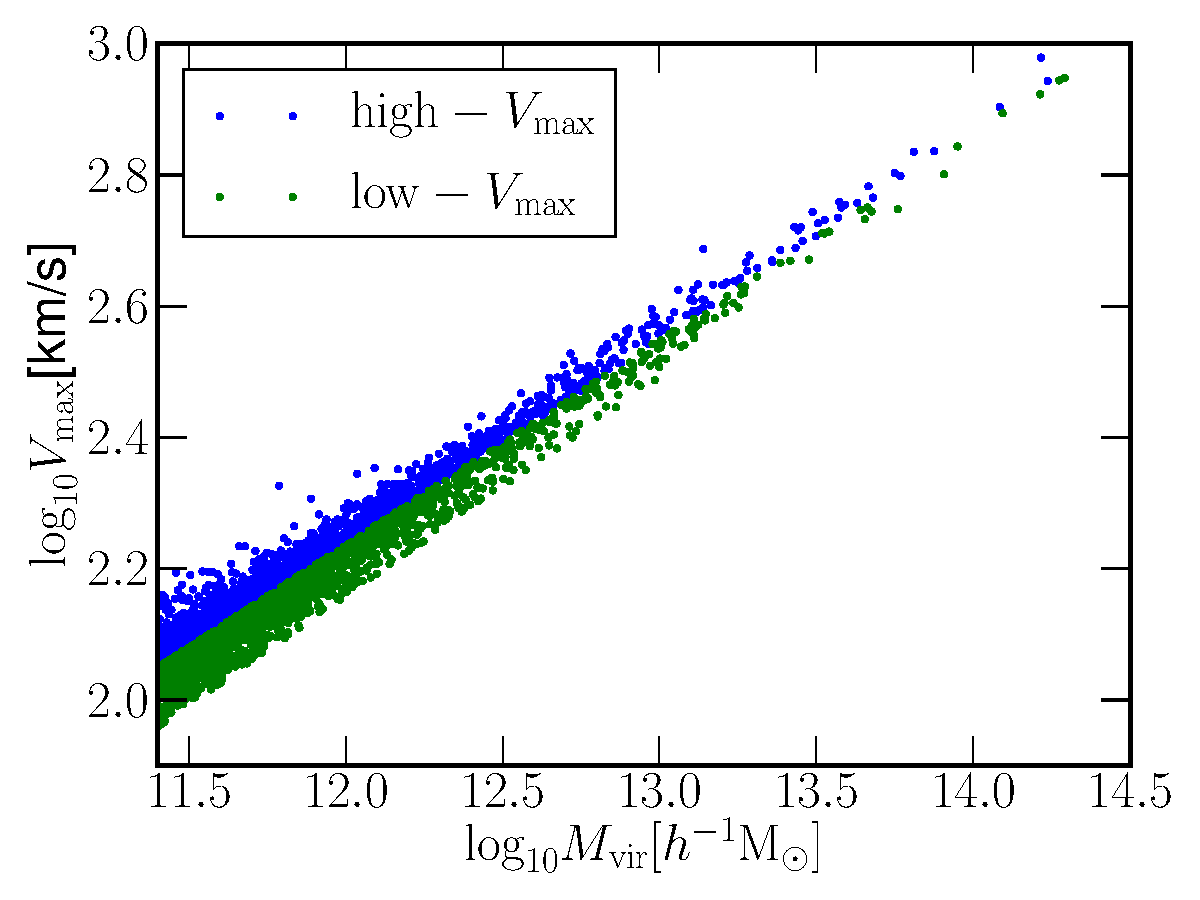
\includegraphics[width=0.5\columnwidth]{\lyxdot \lyxdot /plots/logVmax_logMvir_Dh360}

\caption{\label{fig:vmax-mvir}Distribution of halo mass and the maximum circular
velocity at $z=0.0$ from the MultiDark simulation. The red solid
line represents the maximum circular velocity computed for a given
halo mass using Eq. \ref{eq:vmax-mvir}. The red and green dashed
lines are $1\sigma$ and $2\sigma$ away in the log-normal distribution
of concentration at a fixed halo mass. ??Add color bar to the plot}
\end{figure}


In other words, the above equation is a one to one mapping between
the virial mass of the halo and its maximum circular velocity. Given
this mapping, we can translate clustering measurements as a function
of halo mass into predicted clustering measurements as a function
of maximum circular velocity. Our goal below is to determine whether
this conversion describes the measured clustering or if there is a
residual dependence on the maximum circular velocity. In order to
explore this, we first split the sample into a sequence of virial
mass bins, chosen such that there are the same numbers of halos in
each bin. This process is reminiscent of an abundance-matching procedure
(cite XXX). We then further split each bin into two subsamples with
their observed $V_{{\rm max,obs}}$ greater than (denoted by ``upper'')
or less than (denoted as ``lower'') $V_{{\rm max}}(M_{{\rm vir}})$.
This selection ensures that both the upper and lower subsamples have
the same mean halo mass. Therefore, in the absence of an additional
$V_{{\rm max}}$ dependence (??isn't this $M_{{\rm vir}}$ dependence?)
on clustering, these samples should have the same clustering properties.
Note that this would not be true if we had simply split the sample
along $V_{{\rm max}}$, since the two resulting subsamples would have
different mean halo masses. 

In order to measure halo biases, we compute halo-matter cross correlation
functions for each subsample and measure a linear bias 
\begin{equation}
b_{lin}=<\xi_{hm}(r)/\xi_{mm}(r)>,
\end{equation}
where $\xi_{hm}$ and $\xi_{mm}$ are halo-matter and matter-matter
correlation functions and we take the average of the ratio on $r$
from $10h^{-1}{\rm Mpc}$ to $20h^{-1}{\rm Mpc}$ (??may change to
jackknife samplings). Here, instead of using full DM particles, we
subsample $1000000$ particles to compute matter auto correlation
functions. The reason we use cross correlation functions is to reduce
the shot noise effect on the error.

In Fig. \ref{fig:linear-bias}, we show how linear biases depend on
the maximum circular velocity as a function of halo mass. We compute
linear biases for each mass bin classifying into ``upper'' and ``lower''
maximum circular velocity halos. The halos which have different maximum
circular velocity clearly cluster differently. Furthermore, the relative
bias of ``upper'' versus ``lower'' subsamples increases with decreasing
halo mass to almost 40\% on low mass end.

{*}need some explanations for the decrease of the relative bias on
the lowest mass end? is it real or artificial?

{*}use M{*}

{*}use jackknife sampling to put error bars

{*}where this trend comes from?...assembly bias: concentration?->z\_form

\begin{figure}
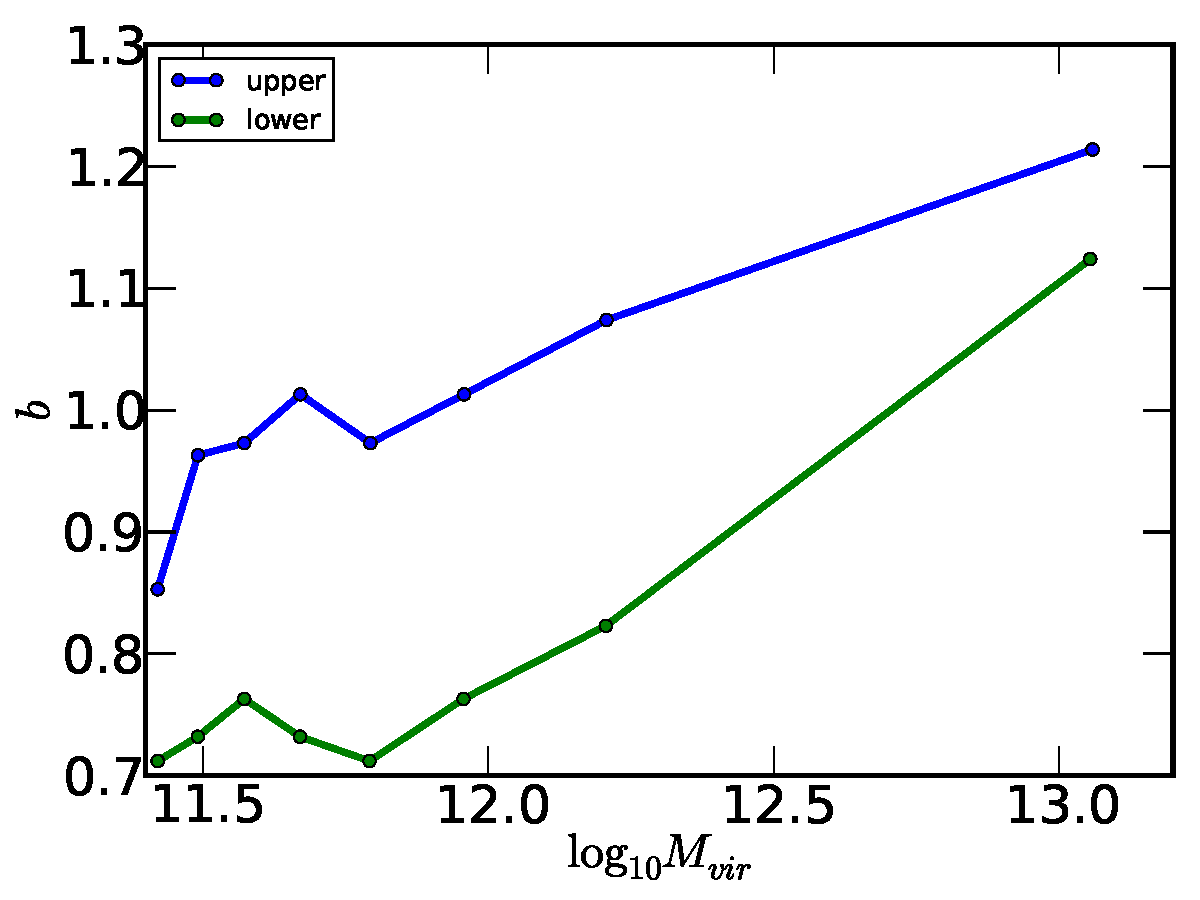
\includegraphics[width=0.5\columnwidth]{\lyxdot \lyxdot /plots/linearBias_wang2_Bolshoi}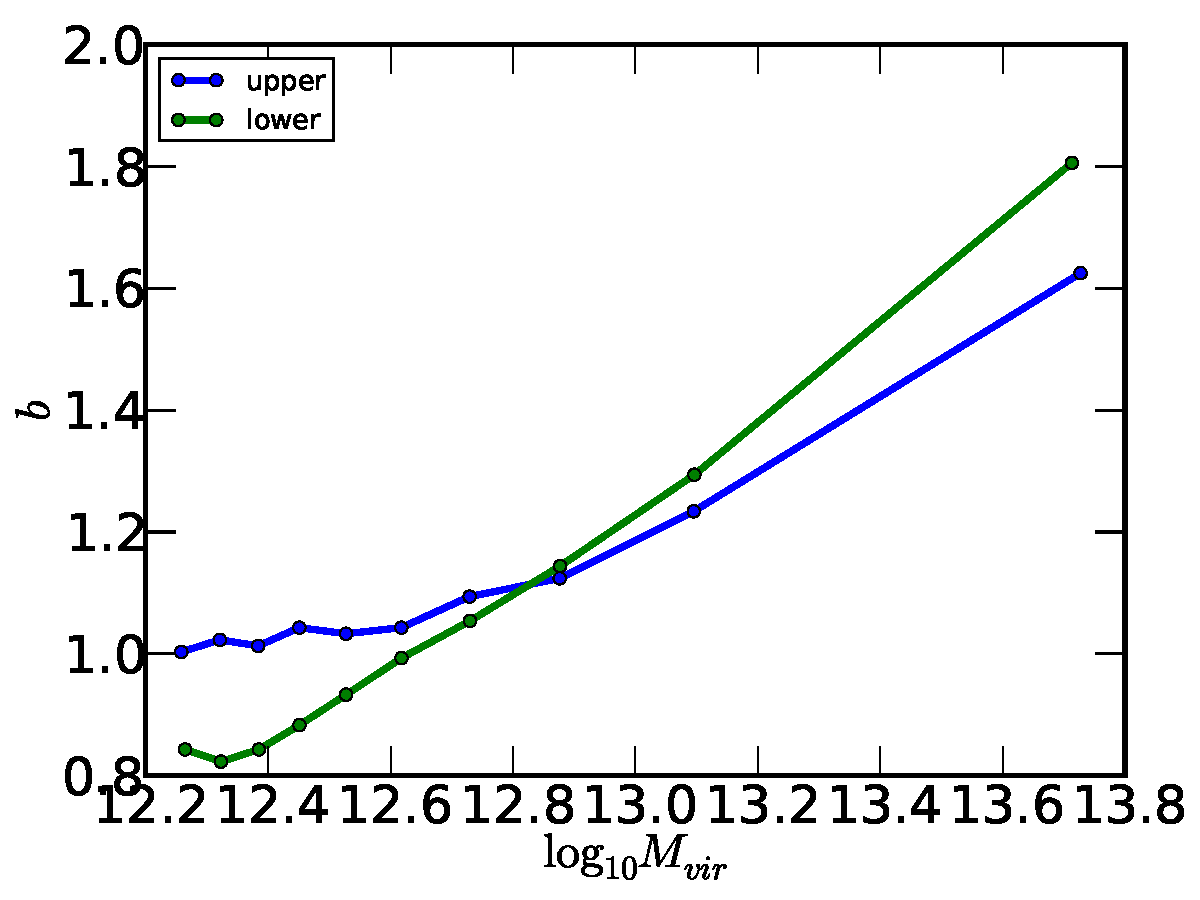
\includegraphics[width=0.5\columnwidth]{\lyxdot \lyxdot /plots/linearBias_wang2_MultiDark}

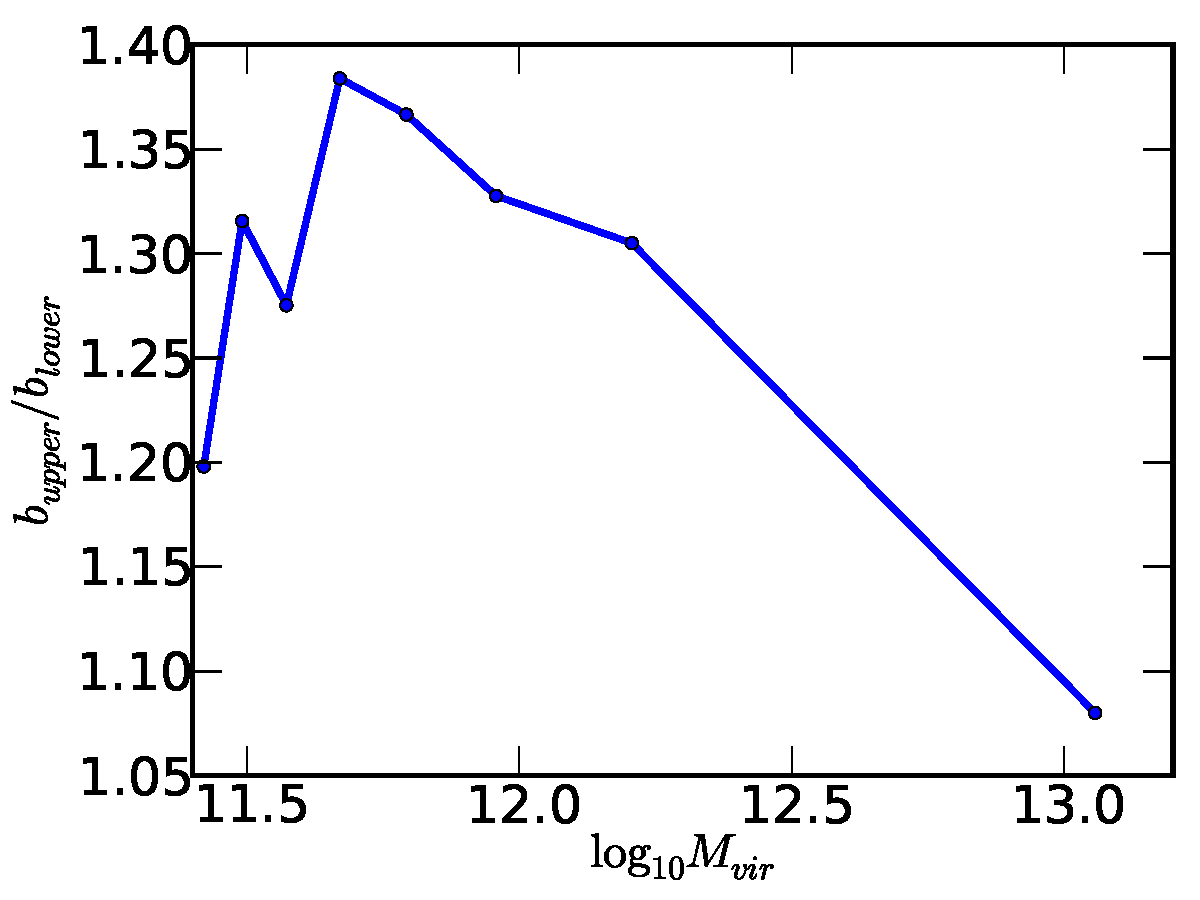
\includegraphics[width=0.5\columnwidth]{\lyxdot \lyxdot /plots/linearBiasRatio_wang2_Bolshoi}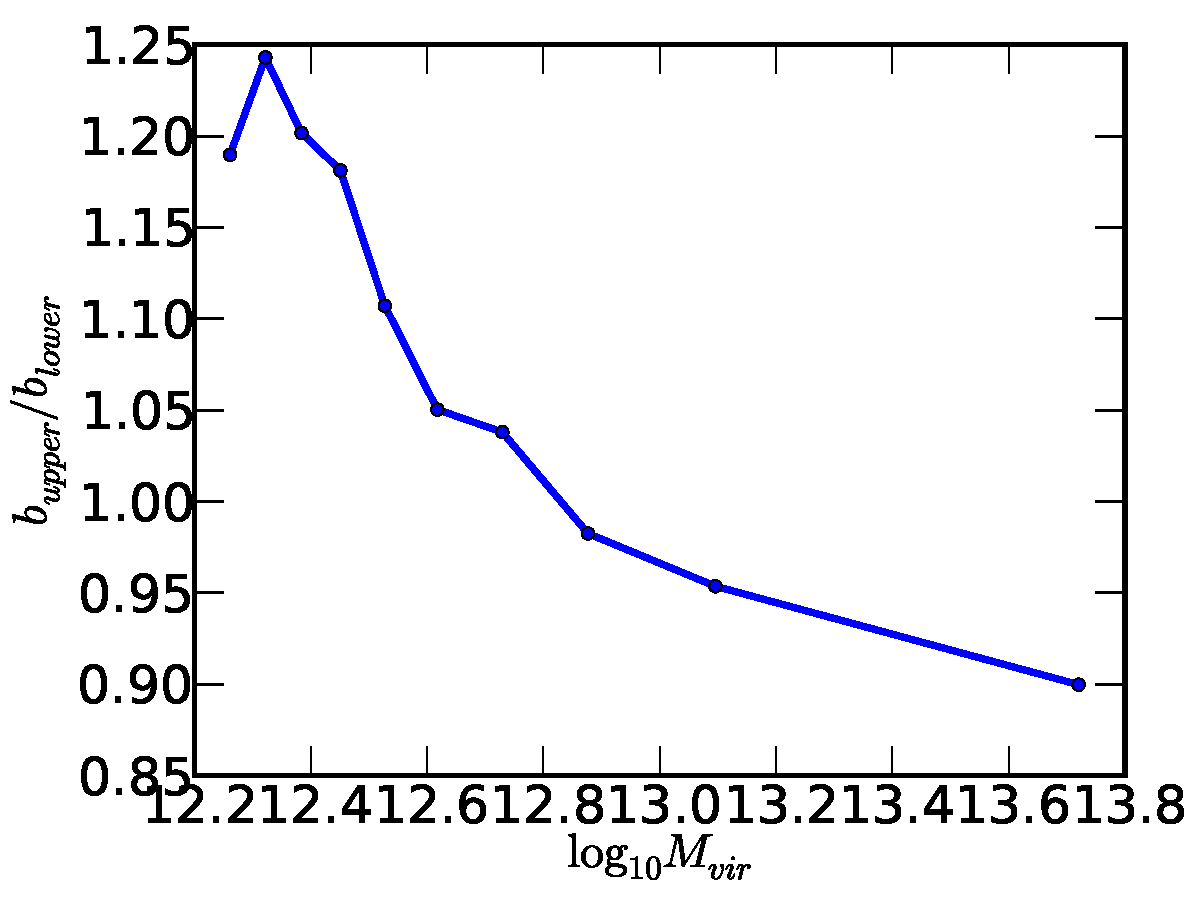
\includegraphics[width=0.5\columnwidth]{\lyxdot \lyxdot /plots/linearBiasRatio_wang2_MultiDark}

\caption{\label{fig:linear-bias}Upper panel: Linear bias at $z=0.0$ as a
function of halo mass from the Bolshoi simulation (left) and the MultiDark
simulation (right). The blue solid line represents a linear bias for
halos whose maximum circular velocities are greater than $V_{{\rm max}}(M_{{\rm vir}})$
from Eq. \ref{eq:vmax-mvir} (labeled as ``upper''), while the green
solid line corresponds to halos whose maximum circular velocities
are smaller than $V_{{\rm max}}(M_{{\rm vir}})$ (labeled as ``lower'').
Lower panel: Ratio of linear biases between ``upper'' and ``lower''
maximum circular velocity halos at $z=0.0$ from the Bolshoi simulation
(left) and the MultiDark simulation (right). As halo masses decrease,
the difference on halo bias between ``upper'' and ``lower'' subsamples
becomes larger.}
\end{figure}


In Fig. \ref{fig:small-scale}, we investigate the maximum circular
velocity dependence of halo bias on small scales. On small scales,
a halo bias is scale-dependent. The question here is whether halos
with different maximum circular velocity have different scale-dependence
on their biases. In order to find that, we take the ratio of halo-matter
cross correlation functions between ``upper\textquotedbl{} and ``lower\textquotedbl{}
subsamples and normalize it by their linear biases. Fig. \ref{fig:small-scale}
clearly shows that the scale-dependence depends on the maximum circular
velocity and its Vmax-dependence is mass-dependent. As halo mass decreases,
the relative scale-dependence between ``upper\textquotedbl{} and
``lower\textquotedbl{} subsamples increases, especially halos with
large maximum circular velocities heavily clustered around $1h^{-1}{\rm Mpc}$. 

{*}Why is upper subsample clustered around 1Mpc/h? Are there any physical
reasons?

{*}Do we get the same scale-dependence by eliminating ejected halos?

\begin{figure}
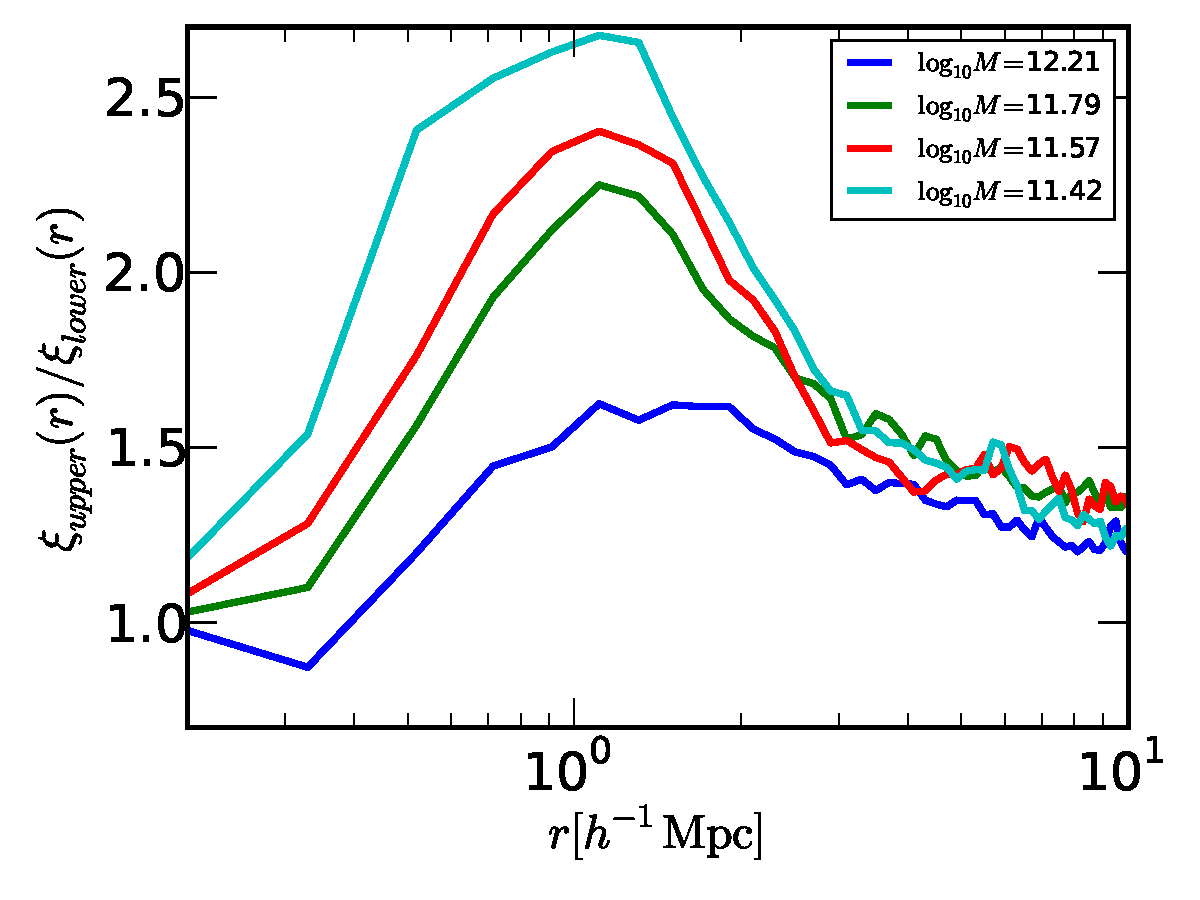
\includegraphics[width=0.5\columnwidth]{\lyxdot \lyxdot /plots/Bolshoi_smallScale_wang2}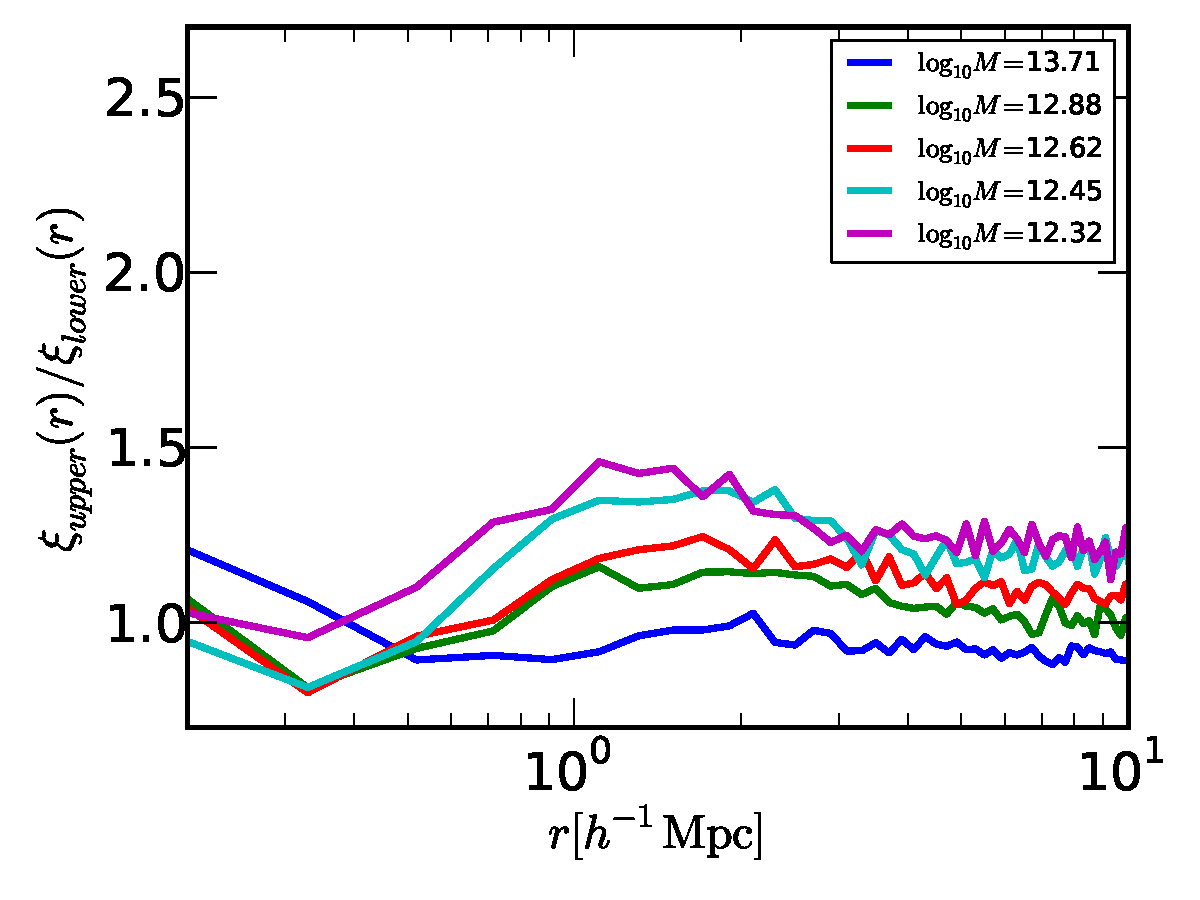
\includegraphics[width=0.5\columnwidth]{\lyxdot \lyxdot /plots/MultiDark_smallScale_wang2}

\caption{\label{fig:small-scale}Ratio of halo-matter cross correlation functions
for \textbackslash{}upper\textquotedbl{} and \textbackslash{}lower\textquotedbl{}
subsamples on small scales normalized by their linear biases. The
plots are from the Bolshoi simulation (left) and the MultiDark simulation
(right) at z = 0:0. Each line corresponds to different halo mass bins
labeled in the plots. Those plots show that \textbackslash{}upper\textquotedbl{}
and \textbackslash{}lower\textquotedbl{} subsamples have dierent scale-dependence
on small scales and the relative scale-dependence between those subsamples
increases smoothly with decreasing halo mass. (?? normalize by their
linear biases)}


\end{figure}



\section{Discussion}
\end{document}
